\documentclass[a4paper,12pt,twoside,openany]{report}

\usepackage{polski}
\usepackage{helvet}
\usepackage[T1]{fontenc}
\usepackage{anyfontsize}
\usepackage[utf8]{inputenc}
\usepackage[pdftex]{graphicx}
\usepackage{tabularx}
\usepackage{array}
\usepackage[polish]{babel}
\usepackage{subfigure}
\usepackage{amsfonts}
\usepackage{verbatim}
\usepackage{indentfirst}
\usepackage[pdftex]{hyperref}
\usepackage{amsmath}
\usepackage{amsfonts}
\usepackage{amssymb}
\usepackage{textcomp}
\usepackage{float}

\raggedbottom

% rozmaite polecenia pomocnicze
% gdzie rysunki?
\newcommand{\ImgPath}{.}

% oznaczenie rzeczy do zrobienia/poprawienia
\newcommand{\TODO}{\textbf{TODO}}


% wyroznienie slow kluczowych
\newcommand{\tech}{\texttt}

% na oprawe (1.0cm - 0.7cm)*2 = 0.6cm
% na oprawe (1.1cm - 0.7cm)*2 = 0.8cm
%  oddsidemargin lewy margines na nieparzystych stronach
% evensidemargin lewy margines na parzystych stronach
\def\oprawa{1.05cm}
\addtolength{\oddsidemargin}{\oprawa}
\addtolength{\evensidemargin}{-\oprawa}

% table span multirows
\usepackage{multirow}
\usepackage{enumitem}	% enumitem.pdf
\setlist{listparindent=\parindent, parsep=\parskip} % potrzebuje enumitem

%%%%%%%%%%%%%%% Dodatkowe Pakiety %%%%%%%%%%%%%%%%%
\usepackage{prmag2017}   % definiuje komendy opieku,nrindeksu, rodzaj pracy, ...


%%%%%%%%%%%%%%% Strona Tytułowa %%%%%%%%%%%%%%%%%
% To trzeba wypelnic swoimi danymi
\title{Predykcja poziomu zapylenia powietrza w Warszawie}

% autor
\author{Mateusz Gierlach}
\nrindeksu{270746}


\opiekun{dr inż. Grzegorz Sarwas}
\terminwykonania{28 lutego 2018} % data na oświadczeniu o samodzielności
\rok{2018}


% To sa domyslne wartosci
% - mozna je zmienic, jesli praca jest pisana gdzie indziej niz w ZETiIS
% - mozna je wyrzucic jesli praca jest pisana w ZETiIS
\miasto{Warszawa}
\uczelnia{POLITECHNIKA WARSZAWSKA}
\wydzial{WYDZIAŁ ELEKTRYCZNY}
\instytut{INSTYTUT STEROWANIA I ELEKTRONIKI PRZEMYSŁOWEJ}
\zaklad{ZAKŁAD STEROWANIA}
\kierunekstudiow{INFORMATYKA}

% domyslnie praca jest inzynierska, ale po odkomentowaniu ponizszej linii zrobi sie magisterska
%\pracamagisterska
%%% koniec od P.W

%\opinie{%
%  \newpage
\begin{center}
 {\large\bf  Opinia} \\
o pracy dyplomowej magisterskiej wykonanej przez dyplomanta\\
{\bf Zdolnego Studenta i Pracowitego Kolegę} \\
 Wydział Elektryczny, kierunek Informatyka,  Politechnika Warszawska\\
Temat pracy\\
\textit{\bf
TYTUŁ PRACY DYPLOMOWEJ
}\\
\end{center}
\medskip
\noindent
Promotor: {\bf dr inż. Miły Opiekun}\\
Ocena pracy dyplomowej: {\bf bardzo dobry}

\medskip

\centerline{\bf Treść opinii}
   Celem pracy dyplomowej panów dolnego Studenta i Pracowitego Kolegi  było
opracowanie systemu pozwalającego symulować  i opartego o oprogramowanie o
otwartych źródłach (ang. Open Source). Jak piszą Dyplomanci, starali się opracować
system, który łatwo będzie dostosować do zmieniających się dynamicznie wymagań,
będzie miał niewielkie wymagania sprzętowe i umożliwiał dalszą łatwą rozbudowę oraz
dostosowanie go do potrzeb.
Przedstawiona do recenzji praca składa się z krótkiego wstępu jasno i
wyczerpująco opisującego oraz uzasadniającego cel pracy, trzech rozdziałów (2-4)
zawierających opis istniejących podobnych
rozwiązań, komponentów rozpatrywanychjako kandydaci do
tworzonego systemu i wreszcie zagadnień wydajności wirtualnych
rozwiązań. Piąty rozdział to opis przygotowanego przez
Dyplomantów środowiska obejmujący opis konfiguracji
środowiska oraz przykładowe ćwiczenia laboratoryjne. Ostatni
rozdział pracy to opis możliwości dalszego
rozwoju projektu. W ramach przygotowania pracy Dyplomanci zebrali i przedstawili w
bardzo przejrzysty sposób duży zasób informacji, co świadczy o dobrej orientacji
w nowoczesnej i ciągle intensywnie rozwijanej tematyce stanowiącej
zakres pracy i o umiejętności przejrzystego przedstawienia tych
wyników. Praca zawiera dwa dodatki, z których pierwszy obejmuje wyniki
eksperymentów i badań nad wydajnością, a drugi to źródła
skryptów budujących środowisko.

 Dyplomanci dość
dobrze zrealizowali postawione przed nimi zadanie,
wykazali się więc umiejętnością zastosowania w praktyce wiedzy
przedstawionej w rozdziałach 2-4.  Uważam, że cele postawione w założeniach pracy zostały pomyślnie
zrealizowane. Proponuję ocenę bardzo dobrą (5).

\vskip 1cm
{
\raggedleft
(data, podpis)\kern1cm

}
%  \newpage
%  \newpage
\begin{center}
 {\large\bf  Recenzja } \\
pracy dyplomowej magisterskiej wykonanej przez dyplomanta\\
{\bf Zdolnego Studenta i Pracowitego Kolegę} \\
 Wydział Elektryczny, kierunek Informatyka,  Politechnika Warszawska\\
Temat pracy\\
\textit{\bf
TYTUŁ PRACY DYPLOMOWEJ
}\\
\end{center}
\medskip
\noindent
Recenzent: {\bf prof. nzw. dr hab. inż. Jan Surowy}\\
Ocena pracy dyplomowej: {\bf bardzo dobry}
\medskip


\centerline{\bf Treść recenzji}
   Celem pracy dyplomowej panów dolnego Studenta i Pracowitego Kolegi  było
opracowanie systemu pozwalającego symulować  i opartego o oprogramowanie o
otwartych źródłach (ang. Open Source). Jak piszą Dyplomanci, starali się opracować
system, który łatwo będzie dostosować do zmieniających się dynamicznie wymagań,
będzie miał niewielkie wymagania sprzętowe i umożliwiał dalszą łatwą rozbudowę oraz
dostosowanie go do potrzeb.
Przedstawiona do recenzji praca składa się z krótkiego wstępu jasno i
wyczerpująco opisującego oraz uzasadniającego cel pracy, trzech rozdziałów (2-4)
zawierających bardzo solidny i przejrzysty opis: istniejących podobnych
rozwiązań (rozdz. 2), komponentów rozpatrywanychjako kandydaci do
tworzonego systemu (rozdz. 3) i wreszcie zagadnień wydajności wirtualnych
rozwiązań, zwłaszcza w kontekście współpracy  kilku elementów
 sieci (rozdział 4). Piąty rozdział to opis przygotowanego przez
Dyplomantów środowiska obejmujący opis konfiguracji
środowiska oraz przykładowe ćwiczenia laboratoryjne (5 ćwiczeń). Ostatni, szósty
rozdział pracy to krótkie zakończenie, które wylicza także możliwości dalszego
rozwoju projektu. W ramach przygotowania pracy Dyplomanci zebrali i przedstawili w
bardzo przejrzysty sposób duży zasób informacji o narzędziach, Rozdziały 2, 3 i 4 świadczą o dobrej orientacji
w nowoczesnej i ciągle intensywnie rozwijanej tematyce stanowiącej
zakres pracy i o umiejętności syntetycznego, przejrzystego przedstawienia tych
wyników. Drobne  mankamenty tej części pracy to zbyt skrótowe omawianie
niektórych zagadnień technicznych, zakładające dużą początkową wiedzę czytelnika
i dość niestaranne podejście do powołań na źródła.
Utrudnia to w pewnym stopniu czytanie pracy i zmniejsza jej wartość dydaktyczną
(a ta zdaje się być jednym z celów Autorów), ale jest zrekompensowane zawartością
merytoryczną. Praca zawiera dwa dodatki, z których pierwszy obejmuje wyniki
eksperymentów i badań nad wydajnością, a drugi to źródła
skryptów budujących środowisko. Praca
zawiera niestety dość dużą liczbę drobnych błędów redakcyjnych, ale nie wpływają
one w sposób istotny na na jej czytelność i wartość. W całej pracy przewijają
się samodzielne, zdecydowane wnioski Autorów, które są wynikiem własnych i
oryginalnych badań.  Rozdział 5 i dodatki pracy przekonują mnie, że Dyplomanci dość
dobrze zrealizowali postawione przed nimi zadanie. Pozwala to stwierdzić, że
wykazali się więc także umiejętnością zastosowania w praktyce wiedzy
przedstawionej w rozdziałach 2-4. Kończący pracę rozdział szósty świadczy o
dużym (ale moim zdaniem uzasadnionym) poczuciu własnej wartości i jest
świadectwem własnego, oryginalnego spojrzenia na tematykę przedstawioną w pracy
dyplomowej. Uważam, że cele postawione w założeniach pracy zostały pomyślnie
zrealizowane. Proponuję ocenę bardzo dobrą (5).

\vskip 1cm
{
\raggedleft
(data, podpis)\kern1cm

}
%}

\streszczenia{
  \newpage
\begin{center}
\large \bf
PREDYKCJA POZIOMU ZAPYLENIA POWIETRZA W WARSZAWIE
\end{center}

\section*{Streszczenie}
W pracy opisany został problem zapylenia smogowego w obszarach zurbanizowanych oraz został zaproponowany sposób rozwiązania go używając powiązań między zmiennymi pogodowymi i smogowymi. Zrobiony został przegląd literatury dotyczącej dotychczasowych sposobów  rozwiązania tego problemu. Zebrane zostały dane pogodowe i ze wskaźników zapylenia. Przeprowadzona została eksploracyjna analiza danych, w celu wydobycia wiedzy na temat powiązań między pogodą, a zapyleniem. Zbudowany został model wyjaśniający te powiązania. Następnie ten model został przetestowany i przedstawione zostały wyniki. W podsumowaniu autor przedstawił możliwe dalsze kierunki rozwoju pracy.

\bigskip
{\noindent\bf Słowa kluczowe:} Eksploracyjna analiza danych, Uczenie maszynowe, Modelowanie statystyczne, Smog, Zapylenie powietrza

\vskip 2cm


\begin{center}
\large \bf
PREDICTION OF SMOG AIR POLLUTION IN WARSAW
\end{center}

\section*{Abstract}
In the thesis, the problem of smog air pollution in urban regions has been described. The author proposed the possible approach to solving it using the relationships between the weather and pollution data. Author researched the solutions that have been published up to this point. Author gathered the data and went through the process of data mining in order to extract the knowledge. The statistical model have been created that explains the relationships in the data. The model has been tested and the effects have been presented. In the summary, the author have outlined the possible next steps in regard to this work.

\bigskip
{\noindent\bf Keywords:} Data mining, Exploratory data analysis, Machine learning, Statistical modelling, Air pollution

\vfill
}

\begin{document}
\maketitle

%-----------------
% Wstęp
%-----------------
\chapter{Wstęp}

\section{Problem smogu}
Zanieczyszczenie powietrza jest jednym z największych wyzwań w dzisiejszym świecie. Światowa Organizacja Zdrowia oszacowała \cite{z1}, że w samym 2012 roku około 7 milionów osób zmarło na skutek chorób powodowanych przez niską jakość powietrza. 

Powietrze zanieczyszczane jest zarówno w wyniku naturalnych procesów jak i działalności człowieka. W pracy tej poruszony został temat jakim jest zapylenie smogowe w obszarach zubranizowanych (na przykładzie Warszawy). Jest to jeden z podproblemów związanych z zanieczyszczeniem powietrza, który jest powodowany całkowicie przez działalność człowieka.

Smog to charakterystyczna mgła zawierająca pyły, tlenki azotu, tlenki siarki, pierwiastki metali ciężkich, tlenki węgla, ozon czy węglowodory aromatyczne. Do jego powstania konieczna jest bezwietrzna pogoda.

Wyróżniamy 2 rodzaje smogu:
\begin{itemize}
	\item smog kwaśny (in. smog londyński, mgła przemysłowa) - występujecy na obszarach miejskich w okresie zimowym. Jego źródłem są przede wszystkim instalacje grzewcze służące do ogrzewania domów, które używają niskiej jakości paliwa.

	\item smog fotochemiczny (in. smog jasny)  - występujący na obszarach miejskich w okresie letnim w dni o dużym nasłonecznieniu. Powstaje na skutek reakcji chemicznej spalin samochodowych i światła słonecznego.
\end{itemize}

\section{Smog kwaśny w Polsce}

Problem zapylenia smogowego w sezonie zimowym w obszarach miejskich w Polsce jest bardzo poważny - Polska się w czołówce krajów Unii Europejskiej o najbardziej zanieczyszczonym powietrzu. Europejska Agencja Środowiska oszacowała, że w wyniku złej jakości powietrza w Polsce umiera przedwcześnie około 48 tysięcy osób.\cite{z2} Oddychanie powietrzem zawierającym smog wywołuje choroby układu oddechowego, w tym także nowotwory płuc, gardła i krtani.

Jedynym typem smogu z jakim mamy do czynienia w Polsce jest smog typu londyńskiego (kwaśny). Najwyższe stężenia pyłów w Polsce odnotowuje się głównie w województwach śląskim (aglomeracja śląska) oraz małopolskim (Kraków). Wysoki poziom smogu jest też obecny w Warszawie, mimo iż to miasto nie leży w dolinie i przepływ wiatru jest w nim większy.

Zdecydowanie najbardziej wpływowym czynnikiem powodującym smog typu kwaśnego w Polsce jest spalanie niskiej jakości paliwa w instalacjach grzewczych w domach jednorodzinnych. W wielu polskich domach wciąż używane są stare instalacje, które spalają dowolny surowiec energetyczny. Bardzo często spalane są w nich węgiel czy odpady, w których zawarte szkodliwe substancje dostają się do atmosfery.

Wpływ na poziom smogu mają również spaliny samochodowe (szacunkowo 15-20\%).
Dlatego też w centrach miast, gdzie występuje zwiększony ruch uliczny, zapylenie jest zazwyczaj większe.

Wbrew powszechnej opinii o dużym wpływie odpadów przemysłowych na zanieczyszczenie powietrza, jego wpływ w stosunku do powyższych dwóch czynników jest niewielki.

Z racji, iż domy jednorodzinne w klimacie jaki występuje w Polsce są ogrzewane głownie w sezonie zimowym oraz późną jesienią, to właśnie w tym okresie obserwujemy problem zwiększonego smogu.

Poziom zapylenia smogowego może być określany wskaźnikami różnego typu, m.in.: stężenie tlenku siarki SO2, stężenie tlenku azotu NO2, stężenie rtęci, zawartość formaldehydu czy stężenie związków ołowiowych.

Jednak wskaźnikami, które w najbardziej ogólny sposób określają poziom zapylenia są:

\begin{itemize}
	\item PM2,5 - stężenie cząsteczek pyłu zawieszonego o średnicy nie większej niż 2,5 mikrometrów. Są to bardzo małe cząsteczki pyłu wnikające głęboko do płuc i osadzające się na ich pęcherzykach. Określane są jako najbardziej szkodliwe. Są to głównie zanieczyszczenia wtórne z przemian dwutlenku siarki lub azotu.
	
	\item PM10 - stężenie cząsteczek pyłu zawieszonego o średnicy nie większej niż 10 mikrometrów. Pyły tego typu  osadzają się w drogach oddechowych.Są to głównie cząsteczki metali ciężkich.
\end{itemize}

\section{Problem predykcji smogu}

Poziom zapylenia smogowego ma dużą zmienność dobową oraz dużą 
zmienność z dnia na dzień. Poza tym, poziom smogu znacznie różni się między sobą w różnych częściach miasta: w centrum ruch samochodowy jest większy, na dużych osiedlach mieszkalnych wydzielane jest więcej dymu pochodzącego ze spalania. Z powodu tej dużej zmienności w czasie i przestrzeni przewidzenie smogu jest zadaniem niełatwym.

\section{Możliwe aplikacje praktyczne}
Precyzyjnie określona wartość poziomu zapylenia w następnym dniu mogłaby mieć zastosowanie w różnych aplikacjach praktycznych.

Jedną z nich jest system powiadamiania o niebezpieczeństwach. Model użyty w aplikacji, która działa w czasie rzeczywistym pozwalałby na wczesne ostrzeganie o zatruciu powietrza i potencjalną ewakuację ludności z terenów objętych zagrożeniem.

Innym przykładem użycia w praktyce takiego modelu mogłaby być aplikacja, która powiadamia o oczekiwanym zapyleniu powietrza na następny dzień, bazując na prognozie pogody, przez co osoby używające takiej aplikacji miałyby informacje, które pozwoliłyby odpowiedzieć na pytania takie jak: czy wyjście z domu bez maski antysmogowej jest bezpieczne, czy bieganie przy ruchliwej ulicy w następny dzień będzie wiązało się z wdychaniem zanieczyszczonego powietrza itd.

\chapter{Opis pracy inżynierskiej}

\section{Proponowane rozwiązanie problemu predykcji}

W tej pracy inżynierskiej, autor postanowił wykonać model predykcyjny poziomu zapylenia smogowego w Warszawie.

Proponowane rozwiązanie oparte jest na następujących założeniach:

\begin{itemize}
	\item Istnieje zależność między czynnikami pogodowymi oraz poziomem smogu. Stworzony model statystyczny ma opisywać mapowania między przestrzenią danych pogodowych i poziomem zapylenia smogowego w dniu poprzednim, a wektorem opisującym smog w dniu dzisiejszym.
	
	\item Typem problemu rozwiązywanym dzięki modelowaniu jest regresja, gdzie zmienną objaśnianą są liczbowe wartości wskaźników PM2,5 i PM10.
	
	\item Ogrzewanie mieszkań jest czynnikiem mającym największy wpływ na poziom smogu w miastach i jego analiza jest wystarczająca do określenia poziomu zapylenia. Nie biorę pod uwagi pozostałych czynników takich jak spaliny samochodowe czy odpady przemysłowe.
	
	\item Ogrzewanie mieszkań, które jest głównym czynnikiem wywołującym smog, jest zależne od temperatury powietrza - mieszkańcy miast ogrzewają domy tym bardziej im niższa jest temperatura na zewnątrz.
	
	\item Prędkość wiatru ma duży wpływ na zapylenie, ponieważ pył zawieszony utrzymuje się przy pogodzie o niskiej wietrzności.
	
	\item Znana jest wartość smogu w dniu poprzednim (to już się wydarzyło, mogliśmy zmierzyć) oraz dzisiejsze wskaźniki pogodowe.
	
	\item Zapylenie w dniu poprzednim wpływa na dzień dzisiejszy. Mimo dużej zmienności smogu z dnia na dzień, smog nie pojawia się i nie znika w sposób gwałtowny.
	
	\item Pogoda w dniu poprzednim wpływa na decyzje mieszkańców miasta o tym czy dalej ogrzewać mieszkanie. Kaloryfery mogą być poodkręcane przez dłuższe okresy czasu i skręcane dopiero, gdy temperatura się znacznie obniży w przeciągu dłuższym niż 1 dzień.
	
	\item Predykcja rozumiana jest jako przewidzenie wartości poziomu zapylenia smogowego następnym dniu mając wartość smogu z dnia poprzedniego. Teoretycznie zakładam, że wartości pogodowe dla następnego dnia są znane z krótkoterminowych prognoz pogody, które mają dużą sprawdzalność, a dzisiejszy smog jest już zmierzony. W praktyce przewidzenie smogu nie jest oparte o pobieranie prognoz pogody, a o wywołanie modelu na zbiorze testowym zakładając, że nie znamy wartości smogu w tym dniu.
	
	\item Model ma zadanie wyjaśniać jak pogoda wpływa na smog. Głównym celem nie jest uzyskanie jak najlepszego dopasowania modelu do danych, a jego interpretowalność, czyli wyjaśnienie które cechy i w jakim stopniu wpływają na powstawanie smogu.
	
\end{itemize}

\section{Założenia pracy}

W pracy autor skupia się na kilku kluczowych podproblemach:

\begin{enumerate}
	\item Zebranie danych historycznych dotyczących pogody i zapylenia powietrza.
	\item Obróbka danych do postaci pozwalającej na analizę.
	\item Eksploracyjna analiza danych i znalezienie relacji pomiędzy cechami(zmiennymi).
	\item Zbudowanie modelu predykcyjnego z użyciem uczenia maszynowego.	
	\item Testowanie modelu i interpretacja wyników	
\end{enumerate}

Część techniczna została napisana z użyciem języka Python w wersji 3. Zostały użyte następujące biblioteki:

\begin{itemize}
	\item Pandas - przechowywanie danych
	\item NumPy - operacje na macierzach
	\item Matplotlib - wizualizacje danych
	\item Scikit-learn - algorytmy uczenia maszynowego
\end{itemize}

\chapter{Analiza istniejących rozwiązań}

\section{Wprowadzenie do przeglądu literatury}
Większość komercyjnie stosowanych aplikacji służących do informowania o poziomie zapylenia nie wprowadziło funkcjonalności prognozowania zapylenia na przyszłość. Jest to związane z faktem, że poziom zapylenia jest mocno zmienny nawet na małej przestrzeni geograficznej, a więc do precyzyjnego jego określenia konieczne jest wiele punktów pomiarowych na terenie jednego miasta. Do danych tego typu często nie ma dostępu w czasie rzeczywistym, są udostępniane dopiero po czasie.

W literaturze znane są metody predykcji smogu oparte o znajdowanie zależności między czynnikami pogodowymi, a wskaźnikami zapylenia. Powszechnie używanym podejściem jest modelowanie ekonometryczne dla regresji liniowej i samodzielne dopasowywanie zmiennych do modelu. Coraz częściej spotykanym podejściem w ostatnich czasach jest również użycie algorytmów uczenia maszynowego do automatycznego wyszukiwania powiązań. 

W pracy autor wykorzystuje części rozwiązań, które już pojawiły się w innych pracach naukowych. Wprowadzane są też nowe elementy, związane m.in. z inżynierią cech.

W dalszych sekcjach tego rozdziału, autor analizuje dwie prace naukowe, które próbują rozwiązać problem predykcji zanieczyszczenia w niestandardowy sposób oraz porównuje je do zaproponowanego podejścia.

\section{Air pollution prediction via multi-label classification; G. Corani, M. Scanagatta}

W tej pracy\cite{z4} rozwiązywanym problemem była klasyfikacja tego czy poziom zanieczyszczenia powietrza na danym obszarze przekroczy pewien ustalony poziom.

Został użyty łączony klasyfikator wielu zmiennych, dzięki któremu możliwe było modelowanie zależności pomiędzy zmiennymi określającymi zanieczyszczenie ozonem, mierzonymi w różnych stacjach. Ta technika pozwoliła uzyskać lepsze wyniki dzięki znalezieniu relacji wielu zmiennych objaśnianych między sobą, które często mają pewną korelację.

W tym celu został napisany klasyfikator wielu zmiennych oparty o sieć Bayesiańską bazującą na uczeniu strukturalnym. 

Zmiennymi objaśnianymi były wartości wskaźników ozonu w różnych stacjach. Okazało się, że ów klasyfikator łączony osiągnął lepszą predykcję niż szrego oddzielnych modeli dla każdej stacji pomiarowej. Zostały również poznane zależności między pomiarami na stacjach.

Podejście w proponowanym rozwiązaniu w stosunku do zaprezentowanego tutaj:
\begin{itemize}
	\item Prognozowana jest konkretna wartość poziomu smogu, a nie to czy zostanie przekroczona pewna granica
	
	\item Założone jest, że wartości smogu w punktach pomiarowych są od siebie niezależne, korelacja między nimi nie jest poszukiwana
	
	\item Model oparty jest o drzewa losowe, nie o sieć Bayesiańską
\end{itemize}

\section{Data mining methods for prediction of air pollution; K. Siwek, S. Osowski}

W tej pracy\cite{z5} zostały przedstawione techniki eksploracji danych służące predykcji zanieczyszczenia powietrza. W pierwszej części został opisany problem generacji i wyboru zmiennych objaśniających, w drugiej części system prognozujący zanieczyszczenie na następny dzień. 

Jako zmienne objaśniające zostały wybrane parametry atmosferyczne. Zmiennymi objaśnianymi są wartości PM10, SO2 (tlenek siarki), NO2 (tlenki azotu) i O3 (ozon).

Użyte są 2 techniki służące do wyboru optymalnych zmiennych do modelu: podejście globalne oparte o analizę całego zbioru danych oraz liniowa metoda stopniowego dopasowania do danych.

Przedstawione są również 2 podejścia do modelowania zależności między zmiennymi meteorologicznymi, a smogowymi. Pierwszą z nich są lasy losowe jako ensembling drzew decyzyjnych, drugą są predyktory oparte o sieć neuronową. Ostatecznie łączone są oba modele.

Praca wykazuje, że dzięki użyciu algorytmów optymalizujących do wyboru cech modelu oraz łączenia podejść tradycyjnego (RandomForest) i sieci neuronowych, możemy uzyskać znacznie wydajności predykcji zanieczyszcenia powietrza.

Podejście w proponowanym rozwiązaniu w stosunku do zaprezentowanego tutaj:
\begin{itemize}
	\item Algorytm wybierający cechy nie jest używany, a zamiast tego przeprowadzana jest eksploracyjna analizę zależności w danych, aby samodzielnie wybrać je do modelu
	
	\item Nie występuje łączenie modeli lasów losowych z siecią neuronową, ponieważ bardziej interesująca jest interpretowalność wyników i wyciągnięcie logicznych wniosków, a nie jak najwyższa predykcja
	
\end{itemize}


\chapter{Zebranie i przygotowanie danych}

\section{Zebranie danych pogodowych}

Dokładne dane pogodowe ze stacji mierniczych są udostępniane przez Instytut Meteorologii i Gospodarki Wodnej na ich stronie: dane.imgw.pl.

Pobrane zostały 2 paczki synoptycznych danych pogodowych dobowych dla zakresu czasowego od 1.01.2011 do 31.12.2017 zmierzone na stacji badawczej nr 352200375 w Warszawie.

Lokalizacja stacji badawczej:

\begin{figure}[H]
	\begin{center}
		\centering
		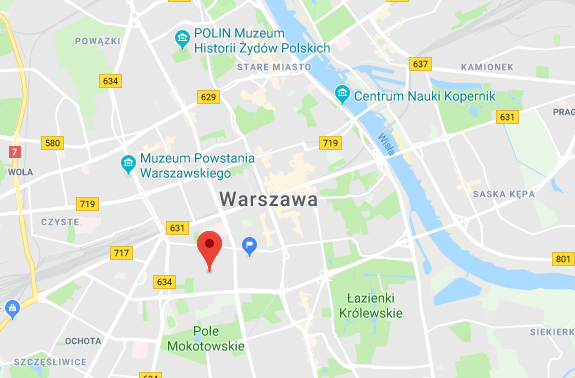
\includegraphics[scale=0.8]{\ImgPath/obr/goegr_pog.png}
	\end{center}
	\caption{Położenie stacji badawczej dla danych pogodowych}
	\label{geogr_stacja}
\end{figure}

1 paczka zawierała następujące zmienne:

\begin{itemize}
	\item Średnie dobowe zachmurzenie ogólne
	\item Status pomiaru NOS
	\item Średnia dobowa prędkość wiatru
	\item Status pomiaru FWS
	\item Średnia dobowa temperatura
	\item Status pomiaru TEMP
	\item Średnia dobowe ciśnienie pary wodnej
	\item Status pomiaru CPW
	\item Średnia dobowa wilgotność względna
	\item Status pomiaru WLGS
	\item Średnia dobowe ciśnienie na poziomie stacji
	\item Status pomiaru PPPS
	\item Średnie dobowe ciśnienie na pozimie morza
	\item Status pomiaru PPPM
	\item Suma opadu dzień
	\item Status pomiaru WODZ
	\item Suma opadu noc
	\item Status pomiaru WONO
\end{itemize}

2 paczka zawierała następujące zmienne:

\begin{itemize}
	\item Maksymalna temperatura dobowa
	\item Status pomiaru TMAX
	\item Minimalna temperatura dobowa
	\item Status pomiaru TMIN
	\item Średnia temperatura dobowa
	\item Status pomiaru STD
	\item Temperatura minimalna przy gruncie
	\item Status pomiaru TMNG
	\item Suma dobowa opadu
	\item Status pomiaru SMDB
	\item Rodzaj opadu
	\item Wysokość pokrywy śnieżnej
	\item Status pomiaru PKSN
	\item Równoważnik wodny śniegu
	\item Status pomiaru RWSN
	\item Usłonecznienie
	\item Status pomiaru USL
	\item Czas trwania opadu deszczu
	\item Status pomiaru DESZ
	\item Czas trwania opadu śniegu
	\item Status pomiaru SNEG
	\item Czas trwania opadu deszczu ze śniegiem
	\item Status pomiaru DISN
	\item Czas trwania gradu
	\item Status pomiaru GRAD
	\item Czas trwania mgły
	\item Status pomiaru MGLA
	\item Czas trwania zamglenia
	\item Status pomiaru ZMGL
	\item Czas trwania sadzi
	\item Status pomiaru SADZ
	\item Czas trwania gołoledzi
	\item Status pomiaru GOLO
	\item Czas trwania zamieci śnieżnej niskiej
	\item Status pomiaru ZMNI
	\item Czas trwania zamieci śnieżnej wysokiej
	\item Status pomiaru ZMWS
	\item Czas trwania zmętnienia
	\item Status pomiaru ZMET
	\item Czas trwania wiatru >=10m/s
	\item Status pomiaru FF10
	\item Czas trwania wiatru >15m/s
	\item Status pomiaru FF15
	\item Czas trwania burzy
	\item Status pomiaru BRZA
	\item Czas trwania rosy
	\item Status pomiaru ROSA
	\item Czas trwania szronu
	\item Status pomiaru SZRO
	\item Wystąpienie pokrywy śnieżnej
	\item Status pomiaru DZPS
	\item Wystąpienie błyskawicy
	\item Status pomiaru DZBL
	\item Stan gruntu Z/R
	\item Izoterma dolna
	\item Status pomiaru IZD
	\item Izoterma górna
	\item Status pomiaru IZG
	\item Aktynometria
	\item Status pomiaru AKTN
\end{itemize}

\section{Zebranie danych smogowych}

Dane ze wskaźników zapylenia smogowego są udostępniane przez Główny Inspektorat Ochrony Środowiska na stronie: http://powietrze.gios.gov.pl.

Dla zakresu czasowego takiego jak dla danych pogodowych, odczyty były dostępne dla 2 punktów pomiarowych na terenie Warszawy:

\begin{itemize}
	\item Wokalna na Ursynowie
	\item Róg Aleji Niepodległości i Nowowiejskiej na Śródmieściu
\end{itemize}

Pobrałem dane smogowe (PM2,5, PM10) godzinne dla zakresu czasowego od 1.01.2011 do 31.12.2016. Dane dla 2017 roku nie zostały jeszcze udostępnione.

Zmienne smogowe:

\begin{itemize}
	\item PM2,5 dla Wokalnej
	\item PM10 dla Wokalnej
	\item PM2,5 dla Niepodległości
	\item PM10 dla Niepodległości
\end{itemize}

Lokalizacje punktów pomiarowych:

\begin{figure}[H]
	\begin{center}
		\centering
		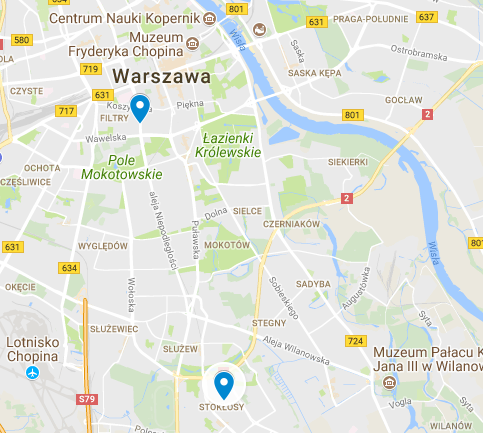
\includegraphics[scale=1]{\ImgPath/obr/geo_smog.png}
	\end{center}
	\caption{Położenie punktów pomiarowych dla danych zapylenia smogowego}
	\label{geogr_smog}
\end{figure}

\section{Obróbka wstępna danych pogodowych}

Z wielu zmiennych, które są w paczkach wybrane zostały tylko te, które mają szanse wyjaśniać smog w jakikolwiek sposób. Kolejnym krokiem jest odrzucenie z 2 paczki zmiennych powtarzających się z 1. Poza tym usunięte zostały zmienne statusowe. Daty rozbite zostały na osobne kolumny: rok, miesiąc, dzień.

Następnie łączone są obie zmienne i usuwane rekordy dla roku 2017, ponieważ nie ma danych dla tego zakresu w przypadku zapylenia PM2,5 i PM10.

Po wstępnym przygotowaniu w ramce danych pogodowych zostają następujące zmienne:

\begin{itemize}
	\item rok
	\item miesiac
	\item dzien
	\item max\char`_temp - maksymalna temperatura zarejestrowana danego dnia
	\item min\char`_temp - minimalna temperatura zarejestrowana danego dnia
	\item sr\char`_temp - średnia temperatura w danym dniu
	\item min\char`_temp\char`_grunt - minimalna temperatura przy gruncie zarejestrowana danego dnia
	\item suma\char`_opad - suma opadów w danym dniu
	\item rodz\char`_opad - rodzaj opadów; W - deszcz, S - śnieg
	\item sr\char`_zachm - średnie zachmurzenie w danym dniu
	\item sr\char`_predk\char`_wiatr - średnia prędkość wiatru w danym dniu
	\item sr\char`_cisn - średnie dobowe ciśnienie pary wodnej
	\item sr\char`_wilg - średnia wilgotność w danym dniu
	\item sr\char`_cisn\char`_stacja - średnie ciśnienie atmosferyczne na poziomie stacji pomiarowej
	\item sr\char`_cisn\char`_morze - średnie ciśnienie atmosferyczne na poziomie stacji morza
	\item opad\char`_dzien - suma opadów za dnia (nie podano jak określany dzień/noc)
	\item opad\char`_noc - suma opadów w nocy
\end{itemize}

\section{Obróbka wstępna danych smogowych}

Dane smogowe są godzinne - po 24 rekordy dla każdego dnia. Sprawdzane jest jak wyglądają średnie wartości odczytów smogowych dla obu stacji w zależności od godziny:

\begin{figure}[H]
	\begin{center}
		\centering
		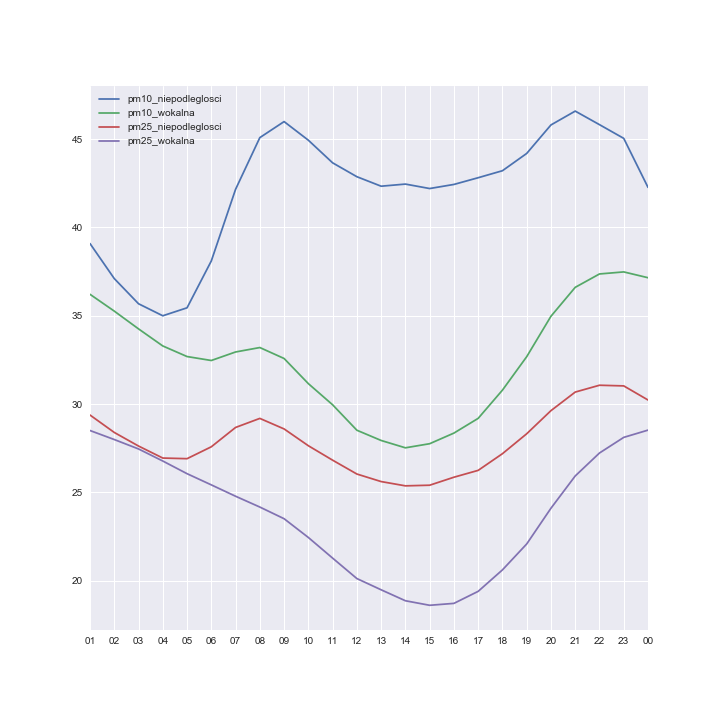
\includegraphics[scale=0.43]{\ImgPath/obr/plot1.png}
	\end{center}
	\caption{Średnie wartości smogu / godzina dnia}
	\label{plot1}
\end{figure}

Zauważmy, że istnieje lokalne maksimum dla godziny 8 rano. Jest to specyficzne miejsce, ponieważ wtedy znaczna część osób mieszkańców Warszawy jedzie samochodami do pracy. Precyzyjne wyjaśnienie wartości w tym miejscu może być ciężkie właśnie ze względu na dodatkowy aspekt zwiększonego ruchu ulicznego w tym czasie, jednak zbudowanie modelu również dla precyzyjnego określenia smogu właśnie dla godziny 8 jest istotne, ponieważ z punktu widzenia praktycznego jest to godzina, dla której chcemy znać dokładnie poziom zapylenia, bo właśnie wtedy wiele osób przemieszcza się po mieście i są szczególnie narażeni na negatywne działanie smogu.

A więc agregując dane godzinne na dni tworzone są zmienne określające wartości PM2,5 i PM10 dla obu punktów pomiarowych (Niepodległości, Wokalna) dla 2 przypadków: wartości średnie z całej doby oraz wartości konkretne dla godziny 8 rano.

Po wstępnym przygotowaniu w ramce danych smogowych zostają następujące zmienne:

\begin{itemize}
	\item rok
	\item miesiac
	\item dzien
	\item pm10\char`_sr\char`_niep - średnia dobowa wartość PM10 na Niepodległości
	\item pm10\char`_sr\char`_wok - średnia dobowa wartość PM10 na Wokalnej
	\item pm25\char`_sr\char`_niep - średnia dobowa wartość PM2,5 na Niepodległości
	\item pm25\char`_sr\char`_wok - średnia dobowa wartość PM2,5 na Wokalnej
	\item pm10\char`_8\char`_niep - wartość PM10 na Niepodległości o 8 rano
	\item pm10\char`_8\char`_wok - wartość PM10 na Wokalnej o 8 rano
	\item pm25\char`_8\char`_niep - wartość PM2,5 na Niepodległości o 8 rano
	\item pm25\char`_8\char`_wok - wartość PM2,5 na Wokalnej o 8 rano
	
\end{itemize}

\chapter{Eksploracyjna analiza danych}

\section{Połączenie danych, brakujące wartości}

Kolejnym krokiem jest sprowadzenie danych do jednej ramki. Łączone są obie ramki po zmiennych czasowych (rok, miesiac, dzien).

Wejściowa ramka danych, na której przeprowadzana jest eksploracja ma 2192 rzędy reprezentujące kolejne dni od 1.01.2011 do 31.12.2016 oraz 25 kolumn reprezentujące zmienne kalendarzowe, pogodowe i smogowe.

Typy i liczności zmiennych:

rok               2192 non-null int64

miesiac           2192 non-null int64

dzien             2192 non-null int64

max\char`_temp          2192 non-null float64

min\char`_temp          2192 non-null float64

sr\char`_temp           2192 non-null float64

min\char`_temp\char`_grunt    2192 non-null float64

suma\char`_opad         2192 non-null float64

rodz\char`_opad         1274 non-null object

sr\char`_zachm          2192 non-null float64

sr\char`_predk\char`_wiatr    2192 non-null float64

sr\char`_cisn           2192 non-null float64

sr\char`_wilg           2192 non-null float64

sr\char`_cisn\char`_stacja    2192 non-null float64

sr\char`_cisn\char`_morze     2192 non-null float64

opad\char`_dzien        2192 non-null float64

opad\char`_noc          2192 non-null float64

pm10\char`_sr\char`_niep      2078 non-null float64

pm10\char`_sr\char`_wok       2175 non-null float64

pm25\char`_sr\char`_niep      2083 non-null float64

pm25\char`_sr\char`_wok       2176 non-null float64

pm10\char`_8\char`_niep       2049 non-null float64

pm10\char`_8\char`_wok        2144 non-null float64

pm25\char`_8\char`_niep       2053 non-null float64

pm25\char`_8\char`_wok        2148 non-null float64

Zauważmy:
\begin{itemize}
	\item rok, miesiac, dzien - typ integer, ale określają klasy - zamieniam na typ kategoryczny
	\item brakujące wartości tylko dla zmiennych smogowych oraz rodz\char`_opad
	\item rodz\char`_opad ma aż 918 brakujących wartości - usuwam kolumnę
\end{itemize}

Następnie analizowane są miejsca, w których występują brakujące wartości dla zmiennych smogowych. Okazuje się, że są to w większości te same rekordy dla różnych zmiennych smogowych. Ponadto zdecydowana większość z nich to brakujące wartości przez wiele rekordów z rzędu, a więc nie ma jak ich zastąpić np. średnią z okolicznych dni. Rekordy z brakującymi wartościami zmiennych smogowych to około 9,5 \% wszystkich rekordów. Zostają usunięte, ponieważ nie spowoduje to drastycznego obniżenia ilości danych.

\section{Korelacje zmiennych}

Niektóre zmienne opisują podobne czynniki. Złą praktyką jest wkładanie do modelu wielu czynników reprezentujących te same informacje pogodowe. Do sprawdzania podobieństw między zmiennymi używana jest korelacji Pearsona. Sprawdzane są korelacje między sobą podobnych zmiennych.

Poniżej przedstawione jest jak prezentują się korelacje między zmiennymi w kilku grupach tematycznych: temperatury, opady, ciśnienia oraz powiązanie opadów z wilgotnością.

\begin{figure}[H]
	\begin{center}
		\centering
		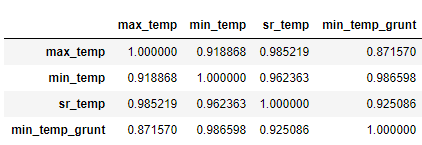
\includegraphics[scale=1]{\ImgPath/obr/temp.png}
	\end{center}
	\caption{Korelacje między temperaturami}
	\label{kortemp}
\end{figure}

\begin{figure}[H]
	\begin{center}
		\centering
		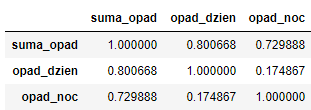
\includegraphics[scale=1]{\ImgPath/obr/opady.png}
	\end{center}
	\caption{Korelacje między opadami}
	\label{korop}
\end{figure}


\begin{figure}[H]
	\begin{center}
		\centering
		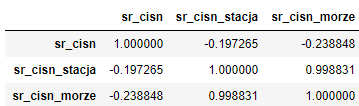
\includegraphics[scale=1]{\ImgPath/obr/cisn.png}
	\end{center}
	\caption{Korelacje między ciśnieniami}
	\label{korcisn}
\end{figure}

\begin{figure}[H]
	\begin{center}
		\centering
		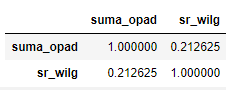
\includegraphics[scale=1]{\ImgPath/obr/op_wilg.png}
	\end{center}
	\caption{Korelacja między opadami, a wilgotnością}
	\label{koropwilg}
\end{figure}

Wyciągane są następujące wnioski:

\begin{itemize}
	\item Temperatury są mocno skorelowane ze sobą - zostawiane są tylko temperaturę średnią, która najlepiej reprezentuje ten czynnik, pozostałe usuwam
	\item Opady w dzień i w nocy nie są skorelowane, ale suma opadów dobrze reprezentuje całość zależności opadów - zostawiane są tylko sumę opadów, pozostałe usuwam
	\item Ciśnienia na poziomie stacji i morza są mocno skorelowane. Zostawiane są ciśnienie na poziomie morza, ponieważ taka informacja jest łatwiejsza do wyciągnięcia np. z prognozy pogody, standardowo ciśnienie podaje się w ten sposób, więc jest to lepiej interpretowalne. Dodatkowo usuwane są średnie ciśnienie pary wodnej, ponieważ w żaden sposób nie powinno wpływać to na smog.
	\item Opady i wilgotność powietrza nie są skorelowane. Zostawiane są obie.
\end{itemize}

Następnie sprawdzana jest korelacja Pearsona między zmiennymi objaśniającymi (pogodą), a objaśnianymi (smogiem). Nie ma tutaj żadnych skorelowanych zmiennych.

Kolejnym krokiem jest sprawdzenie korelacji między zmiennymi objaśnianymi, aby sprawdzić czy smog można reprezentować za pomocą mniejszej liczby zmiennych.

\begin{figure}[H]
	\begin{center}
		\centering
		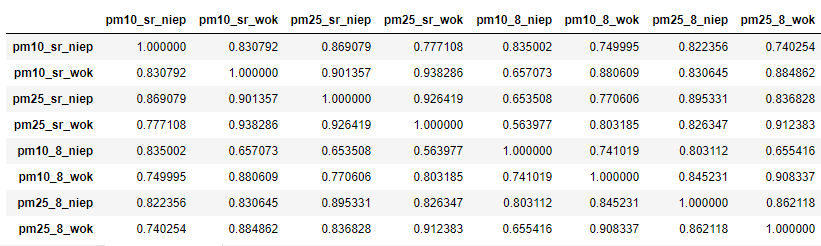
\includegraphics[scale=0.7]{\ImgPath/obr/korobj.png}
	\end{center}
	\caption{Korelacja między zmiennymi objaśnianymi - smogowymi}
	\label{korobj}
\end{figure}

Zauważmy:

\begin{itemize}
	\item Zmienna pm25\char`_8\char`_niep najlepiej reprezentuje dane - jej korelacja z każdą z innych zmiennych nigdy nie jest mniejsza niż 80%
	\item pm10\char`_8\char`_niep i pm25\char`_sr\char`_wok są bardzo słabo skorelowane. Istnieje obawa, że pm25\char`_8\char`_niep niewystarczająco będzie rperezentować różnice w zależnościach między nimi
	\item Ostatecznie: zostawiam 3 zmienne smogowe: pm25\char`_8\char`_niep, pm10\char`_8\char`_niep, pm25\char`_sr\char`_wok - będę robił 3 osobne modele dla tych 3 wskaźników
\end{itemize}

\section{Wartości odstające}

Autor zaczyna od sprawdzenia wartości odstających dla zmiennych objaśniających. Używa w tym celu histogramów, posiłkując się dodatkowo sprawdzaniem ilości wierszy powyżej jakiejś wartości dla konkretnej analizowanej zmiennej.

Histogramy dla zmiennych pogodowych:

\begin{figure}[H]
	\begin{center}
		\centering
		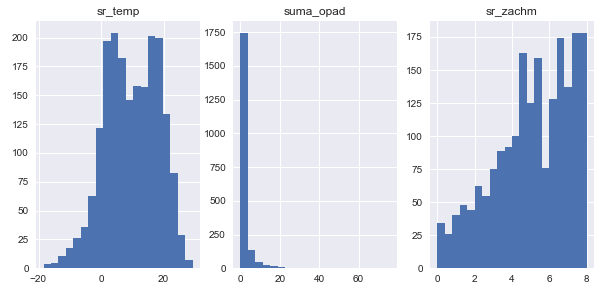
\includegraphics[scale=1]{\ImgPath/obr/hist1.png}
	\end{center}
	\label{hist1}
\end{figure}

\begin{figure}[H]
	\begin{center}
		\centering
		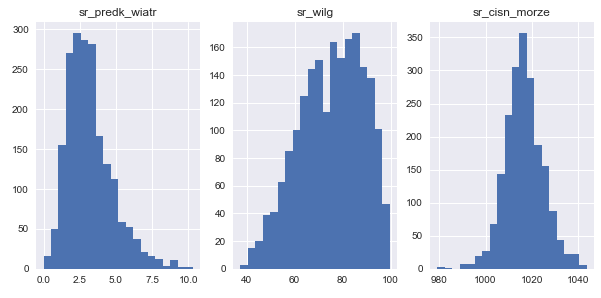
\includegraphics[scale=1]{\ImgPath/obr/hist2.png}
	\end{center}
	\caption{Histogramy dla zmiennych objaśniających}
	\label{hist2}
\end{figure}

Zauważmy, że wartości wyraźnie odstające od trendu są tylko w sumie opadów. Usuwane są rekordy, gdzie wartość tej kolumny jest większa niż 36.

Kolejnym krokiem jest sprawdzenie czy nie występują wartości odstające w zmiennych objaśnianych (zmienne smogowe).

Histogramy dla zmiennych smogowych:

\begin{figure}[H]
	\begin{center}
		\centering
		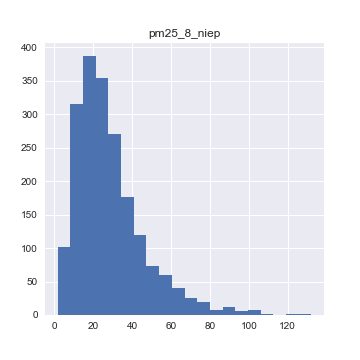
\includegraphics[scale=0.6]{\ImgPath/obr/ho1.png}
	\end{center}
	\label{ho1}
\end{figure}

\begin{figure}[H]
	\begin{center}
		\centering
		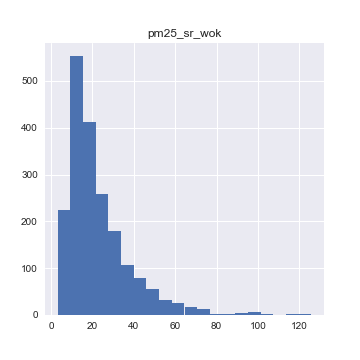
\includegraphics[scale=0.6]{\ImgPath/obr/ho2.png}
	\end{center}
	\label{ho2}
\end{figure}

\begin{figure}[H]
	\begin{center}
		\centering
		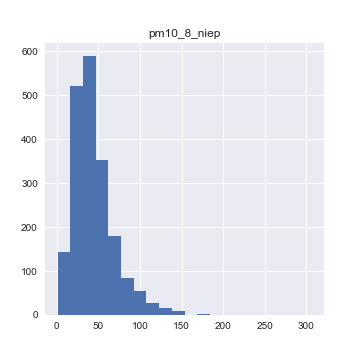
\includegraphics[scale=0.6]{\ImgPath/obr/ho3.png}
	\end{center}
	\label{ho3}
\end{figure}

Zauważmy:

\begin{itemize}
	\item pm25\char`_8\char`_niep ma kilka wartości odstających. Usuwam rekordy dla których zmienna większa od 150.
	\item pm25\char`_sr\char`_wok nie ma wartości odstających.
	\item pm10\char`_8\char`_niep ma wartości odstające, Usuwam rekordy dla których zmienna jest większa pd 180
\end{itemize}

\section{Inżynieria cech}

Oprócz wartości liczbowych zmiennych, ważne jest również by przedstawić w danych pewne dodatkowe aspekty, które mogą polepszyć wyjaśnialność modelu. Przeprowadzany zostaje proces inżynierii cech, czyli tworzenia nowych cech bazując na tych już istniejących.

Nowe zmienne:

\begin{itemize}
	\item bez\char`_wiatru to zmienna boolowska przyjmująca wartość True, jeśli w danym dniu predkosc wiatru była równa 0 i False jeśli różna od 0
	\item poprz\char`_sr\char`_temp to zmienna przechowująca średnią temperaturę z dnia poprzedniego, ponieważ temperatura z dnia wcześniejszego wpływa na to, czy ludzie dalej grzeją w kaloryferach/piecach
	\item Ważne są również zmiany czynników pogodowych z dnia na dzień. To jak zmieniły się czynniki pogodowe z wczoraj na dzisiaj ma wpływ na zachowanie ludzi, jeśli chodzi o ogrzewanie domu. Tak więc tworzony jest szereg nowych zmiennych które są obliczane jako różnica między wartością czynnika z dzisiaj, a wartością z wczoraj. Tworzone są one dla tych czynników: suma opadów, zachmurzenie, prędkość wiatru, wilgotność, ciśnienie atmosferyczne.
\end{itemize}

\section{Smog na przestrzeni lat i miesięcy}

Ważne, by wiedzieć jaki jest trend wartości zapylenia smogowego w zależności od kolejnych lat. Należy sprawdzić czy mam jakiś trend długoterminowy, którego nie dałoby się opisać za pomocą samej pogody i smogu z poprzedniego dnia. Sprawdzany jest on za pomocą wyliczenia średnich wartości zapylenia smogowego dla 3 zmiennych objaśnianych na przestrzeni lat.

\begin{figure}[H]
	\begin{center}
		\centering
		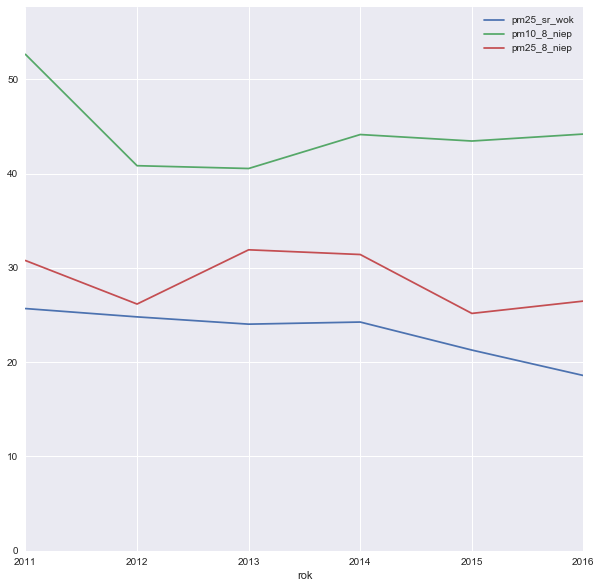
\includegraphics[scale=0.4]{\ImgPath/obr/lata.png}
	\end{center}
	\caption{Średnie zapylenie na przestrzeni lat}
	\label{lata}
\end{figure}

Zauważmy, że nie ma widocznych trendów zmiennych smogowych na przestrzeni lat.

Zobaczmy jak wyglądają uśrednione wartości smogowe na przestrzeni miesięcy. Oczywiste jest, że smog jest duży w sezonie zimowym, ale warto przeanalizować jak to wygląda na wykresie.

\begin{figure}[H]
	\begin{center}
		\centering
		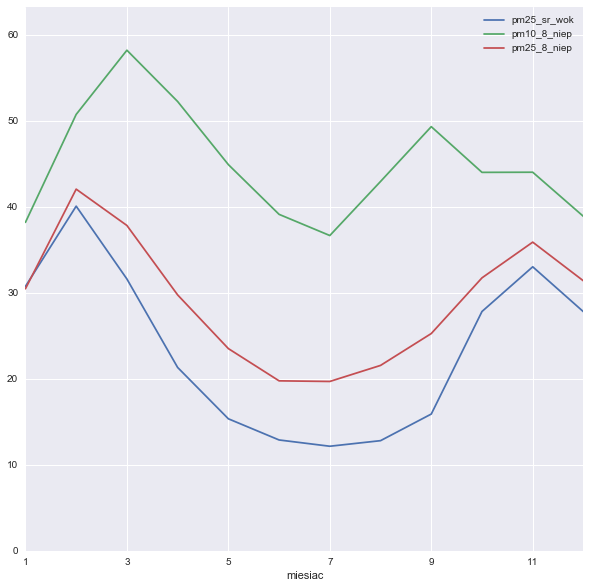
\includegraphics[scale=0.4]{\ImgPath/obr/miesy.png}
	\end{center}
	\caption{Średnie zapylenie na przestrzeni miesięcy}
	\label{miesy}
\end{figure}

Zauważmy, że duże zapylenie jest od października do marca. Zmienna kategoryczna 'miesiac' może w pewien sposób pomagać w predykcji. Autor zostawia ją w ramce i będzie brał ją do modelu.

\section{Zależności między zmiennymi objaśniającymi, a objaśnianymi}

Spodziewamy się, że zmienne objaśniające będą układały się w pewne zależności ze zmiennymi objaśnianymi, np. spodziewane jest, że wraz ze spadkiem temperatury, poziom smogu będzie się zwiększał. Przeanalizujmy wykresy punktowe i sprawdźmy czy rzeczywiście występują jakieś konkretne zależności. Jako zmienną reprezentującą smog wybieram PM2,5 o 8 na Niepodległości, ponieważ jest ona wysoko skorelowana ze wszystkimi innymi wskaźnikami zapylenia.

\begin{figure}[H]
	\begin{center}
		\centering
		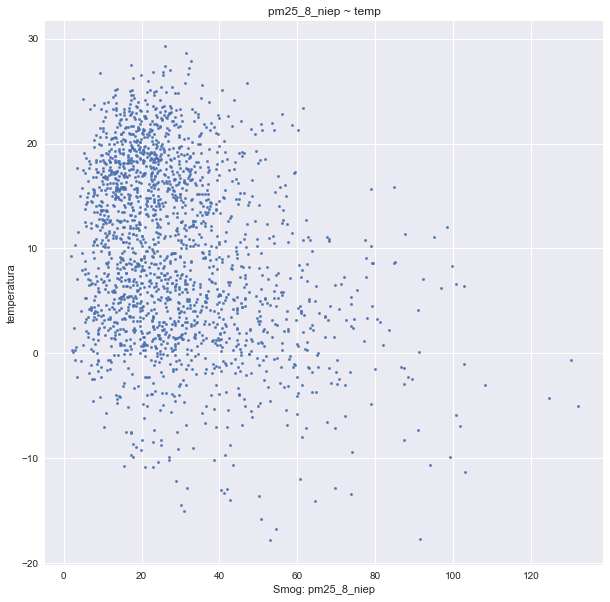
\includegraphics[scale=0.3]{\ImgPath/obr/st.png}
	\end{center}
	\caption{Smog - średnia temperatura}
	\label{st}
\end{figure}

\begin{figure}[H]
	\begin{center}
		\centering
		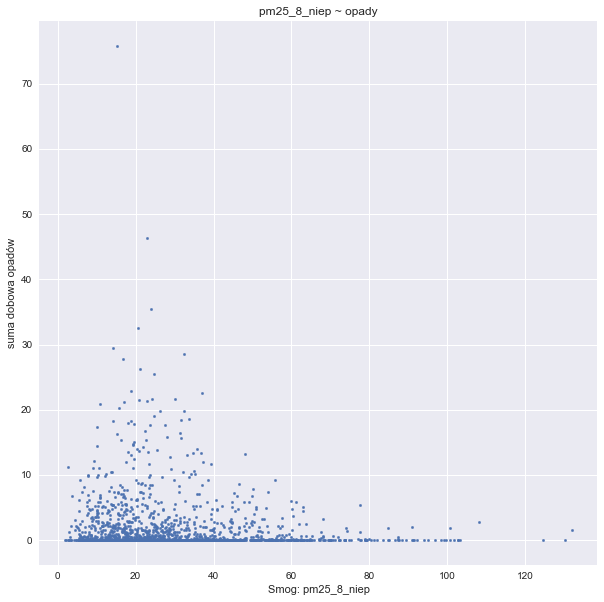
\includegraphics[scale=0.3]{\ImgPath/obr/so.png}
	\end{center}
	\caption{Smog - dobowa suma opadów}
	\label{so}
\end{figure}

\begin{figure}[H]
	\begin{center}
		\centering
		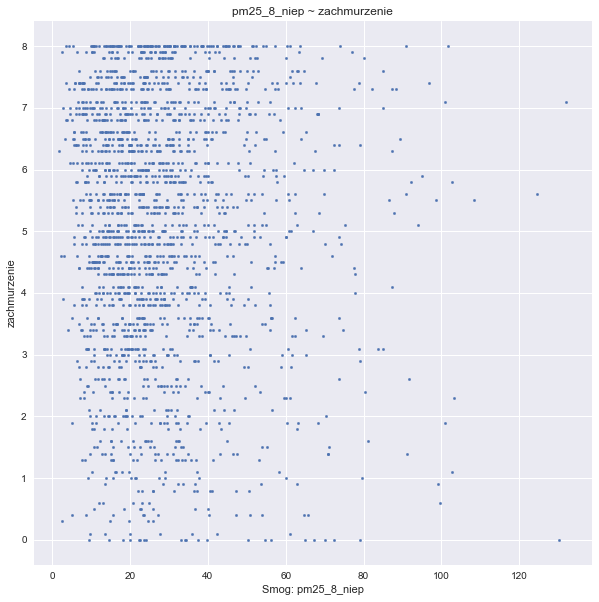
\includegraphics[scale=0.3]{\ImgPath/obr/sz.png}
	\end{center}
	\caption{Smog - średnie zachmurzenie}
	\label{sz}
\end{figure}

\begin{figure}[H]
	\begin{center}
		\centering
		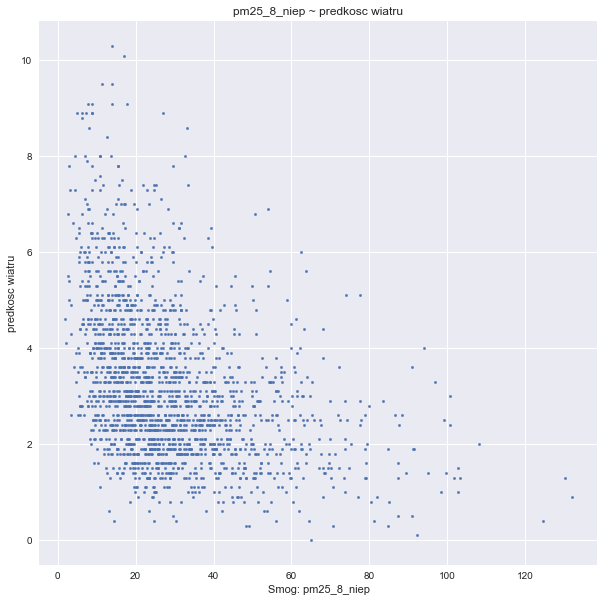
\includegraphics[scale=0.3]{\ImgPath/obr/sw.png}
	\end{center}
	\caption{Smog - średnia prędkość wiatru}
	\label{sw}
\end{figure}

\begin{figure}[H]
	\begin{center}
		\centering
		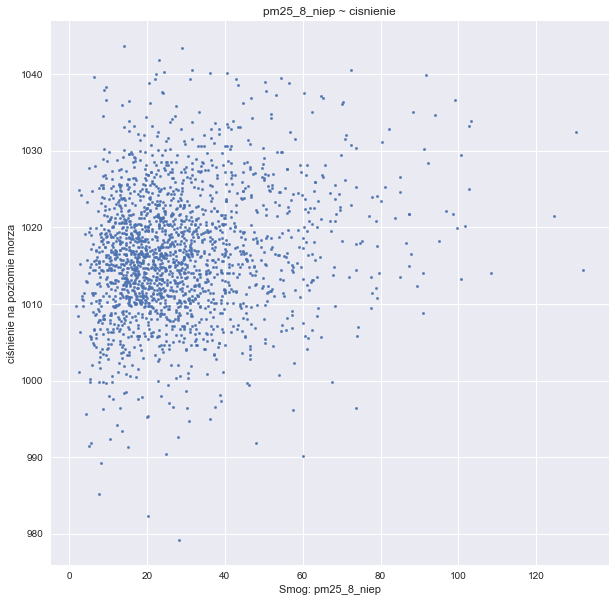
\includegraphics[scale=0.3]{\ImgPath/obr/sc.png}
	\end{center}
	\caption{Smog - średnie ciśnienie na poz. morza}
	\label{sc}
\end{figure}

\begin{figure}[H]
	\begin{center}
		\centering
		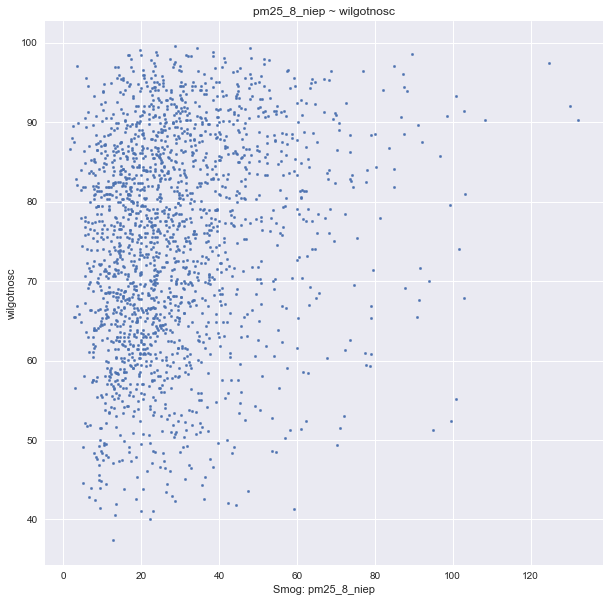
\includegraphics[scale=0.3]{\ImgPath/obr/swi.png}
	\end{center}
	\caption{Smog - średnia wilgotność}
	\label{swi}
\end{figure}


Spostrzeżenia:

\begin{itemize}
	\item Spadek temperatury związany ze wzrostem zapylenia - niewyraźny trend
	\item Brak widocznej zależności między opadami, a smogiem
	\item Brak widocznej zależności między zachmurzeniem, a smogiem
	\item Wraz ze wzrostem prędkości wiatru, smog jest coraz mniejszy - wyraźny trend
	\item Wraz ze wzrostem ciśnienia atmosferycznego, smog również się zwiększa - średni trend
	\item Przy większej wilgotności, smog również zwiększa się w niewielkim stopniu - bardzo słaby trend
\end{itemize}

\section{Skośność rozkładu zmiennych}

Mimo iż algorytm lasów losowych, który jest używany do modelowania dobrze radzi sobie z nierównościami w rozkładzie danych (m.in. dlatego nie przeprowadzam regularyzacji czy standaryzacji zmiennych), to warto "wyrównać" rozkłady niektórych zmiennych, aby zmniejszyć ważność małych wartości i wystarczająca reprezentować też duże wartości zmiennej.

Skośności możemy w łatwy sposób zobaczyć rysując histogramy. Zobaczmy jak wyglądają histogramy wszystkich zmiennych:

\begin{figure}[H]
	\begin{center}
		\centering
		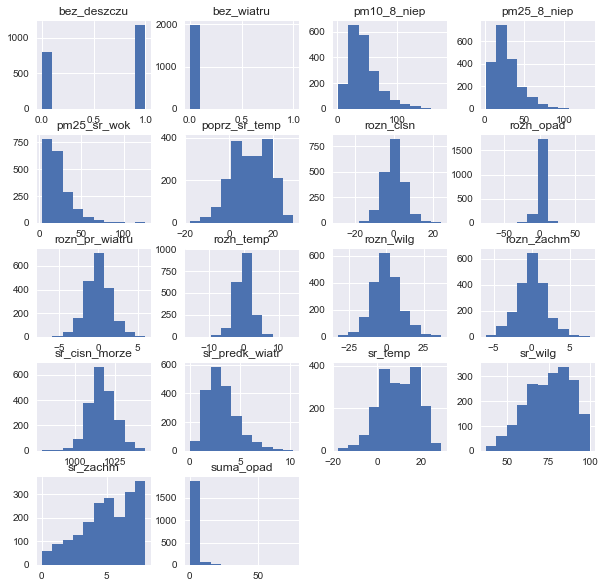
\includegraphics[scale=0.6]{\ImgPath/obr/skews.png}
	\end{center}
	\caption{Histogramy zmiennych}
	\label{skews}
\end{figure}

Zmienne objaśniane o rozkładzie prawoskośnym to suma\char`_opad oraz sr\char`_predk\char`_5wiatr. Logarytmuję je, aby wyrównać rozkłady. Jednak te 2 zmienne zlogarytmowane zostaną podmienione w nowej ramce. Będzie testowane modelowanie na 2 ramkach: ze zmiennymi objaśnianymi zlogarytmowanymi i bez wykonywania tej operacji.

Różnice między rozkładem dla opadów i prędkości wiatru przed i po zlogarytmowaniu:

\begin{figure}[H]
	\begin{center}
		\centering
		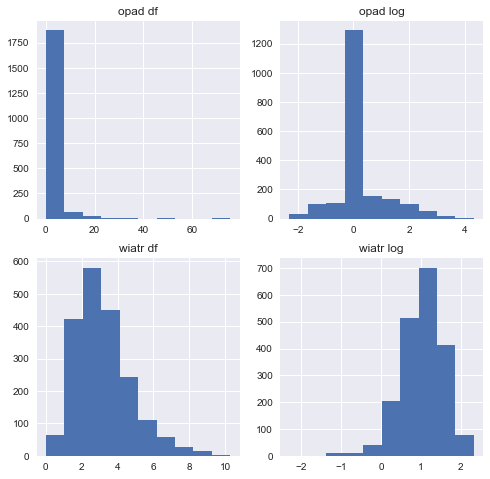
\includegraphics[scale=0.6]{\ImgPath/obr/log-df.png}
	\end{center}
	\caption{Opady i prędkość wiatru przed i po zlogarytmowaniu}
	\label{log-df}
\end{figure}

Następnie autor przechodzi do zmiennych smogowych. Tutaj wszystkie 3 zmienne są wyraźnie prawoskośne. Tutaj również stosowane jest podejście związane z logarytmowaniem i podziale na 2 części (zlogarytmowane, niezlogarytmowane), które będa testowane osobno w modelowaniu.

Tak wyglądają zmienne smogowe po zlogarytmowaniu:

\begin{figure}[H]
	\begin{center}
		\centering
		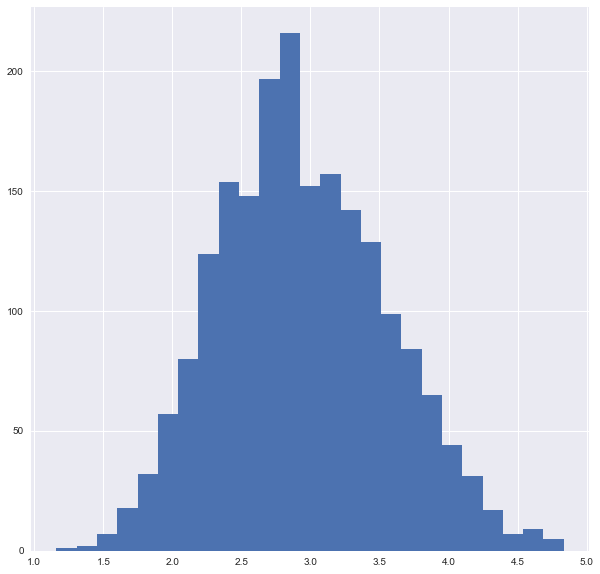
\includegraphics[scale=0.2]{\ImgPath/obr/logo25srwok.png}
	\end{center}
	\caption{PM2,5 średnie Wokalna - po zlogarytmowaniu}
	\label{logo25srwok}
\end{figure}

\begin{figure}[H]
	\begin{center}
		\centering
		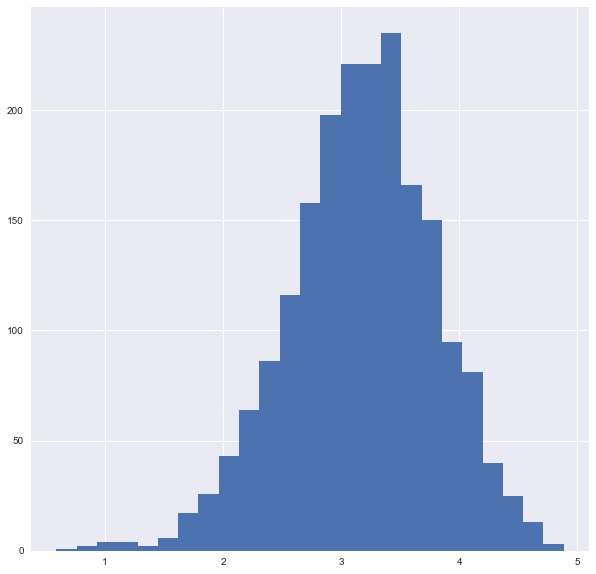
\includegraphics[scale=0.2]{\ImgPath/obr/logo258niep.png}
	\end{center}
	\caption{PM2,5 o 8 Niepodległości - po zlogarytmowaniu}
	\label{logo258niep}
\end{figure}

\begin{figure}[H]
	\begin{center}
		\centering
		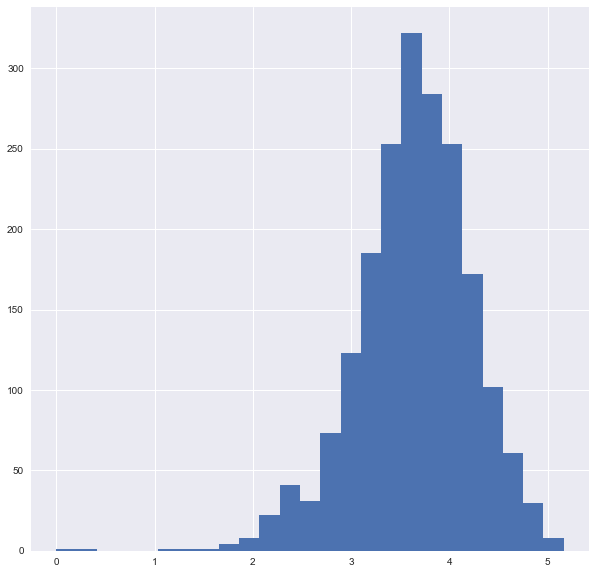
\includegraphics[scale=0.2]{\ImgPath/obr/logo108niep.png}
	\end{center}
	\caption{PM10 o 8 Niepodległości - po zlogarytmowaniu}
	\label{logo108niep}
\end{figure}

Możemy zauważyć wartości odstające w przebiegach. Dopasowywane są do najmniejszej wartości w histogramie, aby na tym etapie nie usuwać zmiennych, bo uniemożliwiło by to porównanie modeli zbudowanych na 2 ramkach.

Tak obrobione dane są gotowe do modelowania.

\chapter{Modelowanie}

Modelowanie jest ostatnim krokiem na drodze do znalezienia powiązań między czynnikami pogodowymi i smogiem. Właściwie zbudowany model jest narzędziem służącym do wyjaśnienia tych powiązań. Sukces etapu modelowania zależy od wcześniejszego poprawnego obrobienia danych, wyboru optymalnego algorytmu do rozwiązywanego problemu oraz umiejętności wyciągnięcia poprawnych wniosków. W tym rozdziale, autor opisuje kolejne etapy składające w procesie modelowania.

\section{Algorytm lasów losowych w problemie regresji}

Do tworzenia modelu wybrany został algorytm lasów losowych dla regresji. Radzi sobie on dobrze zarówno ze zmiennymi ciągłymi jak i kategorycznymi. Nie wymaga skalowania zmiennych w żaden sposób (regularyzacja, standaryzacja itd.) i dzięki wyliczaniu ważności zmiennych daje narzędzie do interpretowanie modelu - ważności zmiennych mówią o tym jak bardzo dana zmienna wpływa na określenie predykcji modelu i pokazuje, które zmienne są najistotniejsze. Lasy losowe są przykładem algorytmu ensemblingowego, który składa się z wielu drzew decyzyjnych. Ilość drzew używanych w modelu jest jedynym modyfikowalnym parametrem.

Poza tym jego dokładność jest bardzo dobra w stosunku do innych tradycyjnych algorytmów uczenia maszynowego. Oczywiście jest mniej dokładny niż np. sieci neuronowe, ale w przypadku tego modelu ważne jest zarówno stosunkowo niezłe dopasowanie jak i wyjaśnialność, czego sieć neuronowa nie zapewnia.

\section{Wstęp do procesu modelowania}

Zanim będą wyciągane wnioski dotyczące całego problemu przewidzenia smogu, autor chce najpierw dzięki procesowi modelowania znaleźć odpowiedzi na następujące pytania:

\begin{itemize}
	\item Czy lepsze jest uczenie na zbiorze ze zmiennymi objaśniającymi zlogarytmowanymi czy na standardowych?
	\item Czy lepiej, aby zmienna objaśniana była zlogarytmowana czy nie?
	\ Czy same czynniki pogodowe są wystarczające, aby dobrze określić predykcję, czy objaśnianie za pomocą smogu w dniu poprzednim jest absolutnie konieczne?
\end{itemize}

Ostatecznie dzięki modelowi autor chce znaleźć odpowiedzi na pytania dotyczące całego procesu predykcji zapylenia smogowego:

\begin{itemize}
	\item Które czynniki pogodowe są najważniejsze?
	\item Czy smog w różnych punktów Warszawy możemy przewidzieć z podobną precyzją?
	\item Czy smog o 8 rano dobrze możemy przewidzieć z podobną predykcją jak uśredniony smog dla całego dnia?
\end{itemize}

Za każdym razem, gdy tworzone są modele, dokonywany jest podział danych na zbiór treningowy i testowy w stosunku 80/20. Modele między sobą są porównywane za pomocą 3 statystyk opisujących zależności między wartościami rzeczywistymi z mierników smogu, które nie zostały użyte do tworzenia modelu (20\%), a predykcją modelu na danych testowych: 

\begin{itemize}
	\item Współczynnik determinacji r-kwadrat (R2) opisujący miarę dopasowania modelu (jest to najważniejsza miara)
	\item Korelacja Spearmana
	\item Korelacja Pearsona
\end{itemize}

\section{Model oparty na samej pogodzie - kwestia logarytmowania}

W pierwszej kolejności tworzony jest model, który opisuje zależność między samymi czynnikami pogodowymi (nie biorąc pod uwagę smogu w dniu poprzednim).

Jest on tworzony po to, aby zobaczyć jak zmienia się predykcja, gdy 2 z czynników pogodowych są logarytmowane. Wykonywane są modele tylko dla 1 zmiennej objaśnianej: pm25\char`_8\char`_niep. Las losowy tworzony jest w oparciu o 500 drzew decyzyjnych.

\textbf{Zmienne pogodowe bez logarytmowania:}

R2 na zb. testowym: 0.485
Kor. Spearmana na zb. testowym: 0.704
Kor. Pearsona na zb. testowym: 0.701

\textbf{Zmienne pogodowe z logarytmowaniem:}

R2 na zb. testowym: 0.488
Kor. Spearmana na zb. testowym: 0.673
Kor. Pearsona na zb. testowym: 0.705

Jak widzimy, logarytmowanie zmiennych objaśniających w prawie żaden sposób nie wpływa na polepszenie modelu. W dalszej części modelowania, używane są tylko ramki danych oparte o standardowe wartości zmiennych pogodowych.

Zauważmy, że poziom predykcji, gdy smog próbujemy objaśniać samą pogodą jest słaby. Pokrycie wartości testowych na poziomie ok. 49\% jest niewystarczające do precyzyjnego przewidzenia wartości smogu.

Na wykresie dokładnie widać jak słabe jest pokrycie (niebieski - wartości prawdziwe, czerwona przerywana - predykcja modelu):

\begin{figure}[H]
	\begin{center}
		\centering
		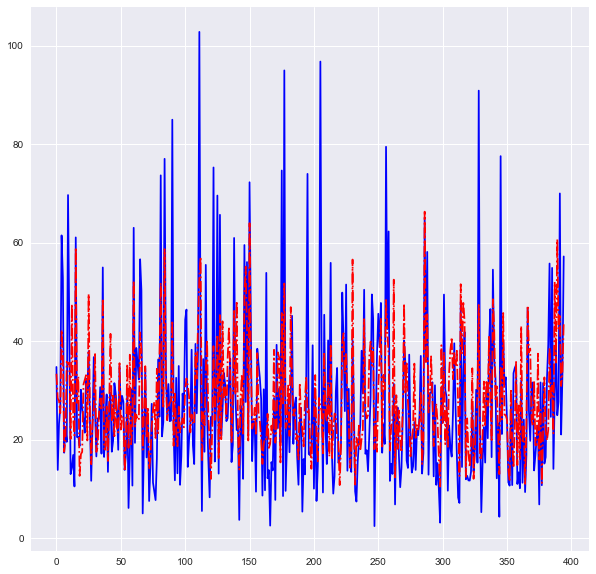
\includegraphics[scale=0.6]{\ImgPath/obr/mbs.png}
	\end{center}
	\caption{Pokrycie modelu bazującego na samych zmiennych pogodowych}
	\label{mbs}
\end{figure}


\section{Model oparty na pogodzie i smogu z dnia poprzedniego - kwestia logarytmowania}

Predykcja smogu oparta na czynnikach pogodowych oraz smogu z dnia poprzednie ma duży sens, ponieważ zakładamy, że smog historyczny jest znany.

Bardzo istotne jest to, że smog z dnia poprzedniego nie jest czynnikiem wyjaśniającym to jaki poziom smogu jest dzisiaj, wyjaśniamy to tylko za pomocą zmiennych pogodowych. Ale wiedząc, że smog nie zmienia się w sposób bardzo gwałtowny, nasza predykcja powinna być dokładniejsza, gdy znamy bazę z dnia poprzedniego, a pogodą staramy się wyjaśnić zmianę zapylenia.

W tym kroku autor chce sprawdzić czy logarytmowanie zmiennych smogowych (zarówno zmienna objaśniana jak i objaśniająca smogowa dla dnia poprzedniego) daje polepszenie predykcji. Znów wykonywane modele tylko dla 1 zmiennej objaśnianej: pm25\char`_8\char`_niep.

\textbf{Zmienne pogodowe bez logarytmowania:}

R2 na zb. testowym:  0.54
Kor. Spearmana na zb. testowym: 0.71
Kor. Pearsona na zb. testowym: 0.737


\textbf{Zmienne pogodowe z logarytmowaniem:}

R2 na zb. testowym: 0.497
Kor. Spearmana na zb. testowym: 0.671
Kor. Pearsona na zb. testowym: 0.699

Zauważmy, że po raz kolejny logarytmowanie nie polepsza modelu, a tutaj wręcz go pogarsza. W dalszej części używane są tylko zmienne niezlogarytmowane.

Dokładając smog z dnia poprzedniego nieznacznie polepszylismy precyzję predykcji modelu.

Wykres modelu bez logarytmowania, widać lekką poprawę w stosunku do poprzedniego:

\begin{figure}[H]
	\begin{center}
		\centering
		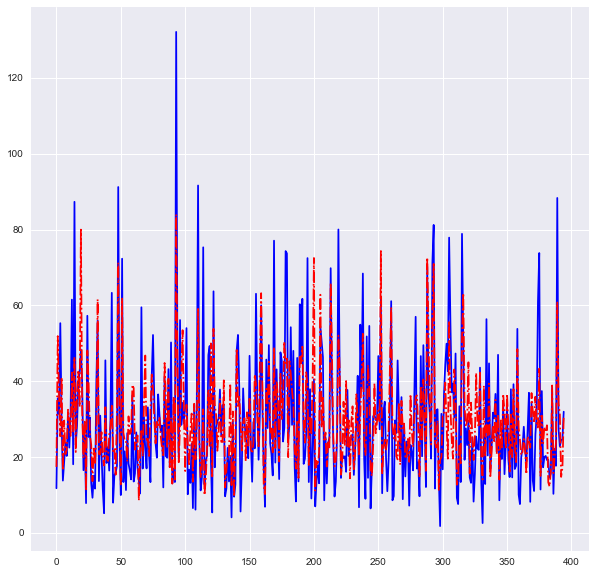
\includegraphics[scale=0.6]{\ImgPath/obr/mod2.png}
	\end{center}
	\caption{Pokrycie modelu bazującego na zmiennych pogodowych i poprzedniej wartości zapylenia}
	\label{mod2}
\end{figure}

\section{Ostateczne modele}
Ostatnim krokiem w modelowaniu jest wykonanie modeli dla 5 wybranych zmiennych objaśnianych:

\begin{itemize}
	\item PM2,5 średnie Wokalna
	\item PM10 o 8 Niepodległości
	\item PM2,5 o 8 Niepodległości
	\item PM10 o 8 Wokalna
	\item PM10 średnie Niepodległości
\end{itemize}

\textbf{PM2,5 średnie Wokalna:}

R2 na zb. testowym: 0.721

Kor. Spearmana na zb. testowym: 0.87

Kor. Pearsona na zb. testowym: 0.849


\textbf{PM10 o 8 Niepodległości:}

R2 na zb. testowym: 0.329

Kor. Spearmana na zb. testowym: 0.527

Kor. Pearsona na zb. testowym: 0.575


\textbf{PM2,5 o 8 Niepodległości:}

R2 na zb. testowym: 0.419

Kor. Spearmana na zb. testowym: 0.647

Kor. Pearsona na zb. testowym: 0.647


\textbf{PM10 o 8 Wokalna:}

R2 na zb. testowym: 0.312

Kor. Spearmana na zb. testowym: 0.603

Kor. Pearsona na zb. testowym: 0.569


\textbf{PM10 średnie Niepodległości:}

R2 na zb. testowym: 0.497

Kor. Spearmana na zb. testowym: 0.736

Kor. Pearsona na zb. testowym: 0.705


Zauważmy:

\begin{itemize}
	\item PM2,5 jest przewidywane trochę lepiej niż PM10
	\item Smog uśredniony dla całego dnia przewidywany lepiej niż dla 8 rano
	\item Smog na Wokalnej przewidywany jest lepiej niż na Niepodległości
\end{itemize}

\chapter{Badanie otrzymanych modeli}

\section{Przedstawienie najlepszego modelu}

Model o największej precyzji predykcji to model dla PM2,5, smogu uśrednionego, mierzonego na Wokalnej.

R2 na zb. testowym: 0.721

Kor. Spearmana na zb. testowym: 0.87

Kor. Pearsona na zb. testowym: 0.849

\begin{figure}[H]
	\begin{center}
		\centering
		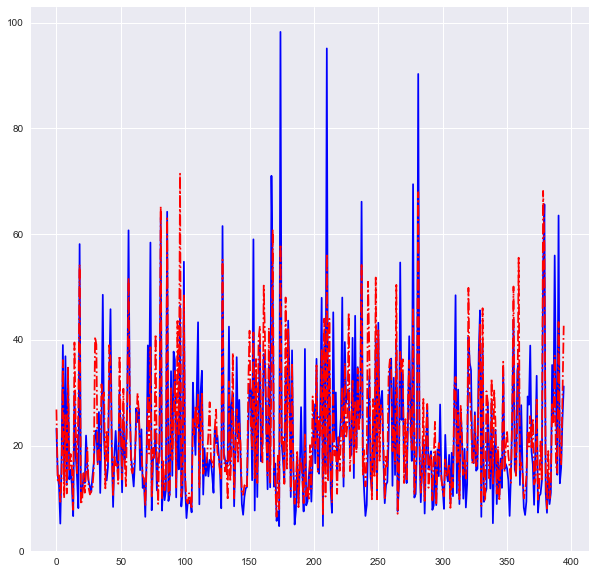
\includegraphics[scale=0.42]{\ImgPath/obr/best.png}
	\end{center}
	\caption{Pokrycie najlepszego modelu}
	\label{best}
\end{figure}

\section{Kros-walidacja modelu}

Testując stworzony model, autor przeprowadził testy kros-walidacyjne, czyli wtórny podział zbioru na treningowy i testowy i wywołanie modelu na nowych danych, sprawdzając jak zmienia się precyzja predykcji.

R2 dla zbiorów treningowych z kros-walidacji - testy przeprowadzone zostały 6 razy:

\begin{itemize}
	\item 0.72253292
	\item 0.66410089
	\item 0.71541177
	\item 0.64480448
	\item 0.72832458
	\item 0.61368826
\end{itemize}

Model ma rzeczywistą predykcję na poziomie ok. 70\%.

\begin{figure}[H]
	\begin{center}
		\centering
		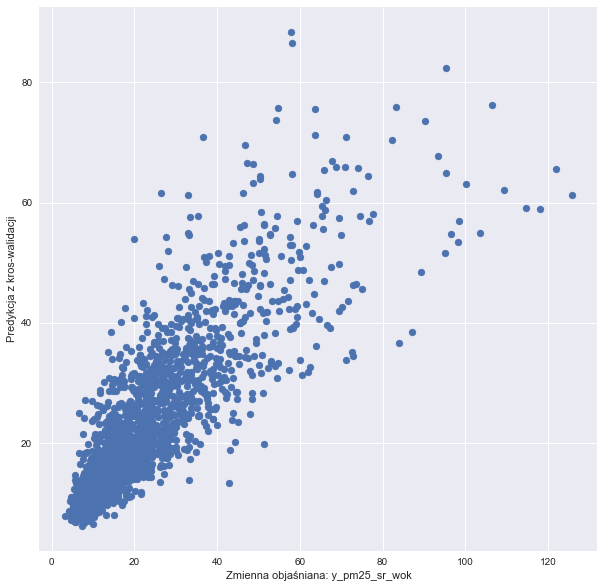
\includegraphics[scale=0.42]{\ImgPath/obr/kros.png}
	\end{center}
	\caption{Predykcja z kros-walidacji - zmienna objaśniana}
	\label{kros}
\end{figure}

\section{Interpretacja modelu predykcji}

Głównym narzędziem interpretacyjnym stworzonego modelu są ważności cech które wchodzą do modelu:

[(0.51849999999999996, 'pop\char`_pm25\char`_sr\char`_wok')

(0.1356, 'sr\char`_predk\char`_wiatr')

(0.059200000000000003, 'poprz\char`_sr\char`_temp')

(0.050700000000000002, 'sr\char`_temp')

(0.042700000000000002, 'rozn\char`_wilg')

(0.030499999999999999, 'sr\char`_cisn\char`_morze')

(0.028199999999999999, 'sr\char`_zachm')

(0.026700000000000002, 'rozn\char`_temp')

(0.024799999999999999, 'rozn\char`_pr\char`_wiatru')

(0.0224, 'rozn\char`_cisn')

(0.0178, 'rozn\char`_zachm')

(0.017000000000000001, 'sr\char`_wilg')

(0.0106, 'rozn\char`_opad')

(0.0085000000000000006, 'miesiac')

(0.0054999999999999997, 'suma\char`_opad')

(0.0011999999999999999, 'bez\char`_deszczu')

(0.0, 'bez\char`_wiatru')]

\section{Wnioski}

Najważniejsze wnioski dotyczące procesu predykcji zapylenia wyciągnięte dzięki modelowaniu:

\begin{itemize}
	\item Prędkość wiatru jest najważniejszym czynnikiem mającym wpływ na poprawną predykcję
	\item Temperatura w dniu analizowanym i w dniu poprzednim to drugi najważniejszy czynnik
	\item Zmiana wilgotności z dnia na dzień również w duży sposób wpływa na predykcję
	\item Ciśnienie atmosferyczne i zachmurzenie mają już mniejszy wpływ, ale też są istotne
	\item Możemy uznać, że pozostałe czynniki nie mają wpływu na predykcję smogu
	\item Łatwiejsze jest prognozowanie smogu w obszarze mieszkalnym (Wokalna na Ursynowie), gdzie ruch uliczny jest mniejszy, a palenie w piecach ma zdecydowanie największy wpływ na smog, niż w obszarze o dużym ruchu ulicznym (Niepodległości), ponieważ nie mam jak "uchwycić" tego czynnika w modelu
\end{itemize}



\chapter{Podsumowanie}

\section{Wstęp do podsumowania}

Przedmiotem pracy było stworzenie modelu wyjaśniającego jak czynniki pogodowe wpływają na poziom zapylenia smogowego. Stworzony model ma służyć predykcji smogu w analizowanym dniu w oparciu o dane z przeszłości.

Podczas procesu tworzenia pracy, zostały wykonane następujące etapy:

\begin{enumerate}
	\item Zebranie danych historycznych dotyczących pogody i zapylenia powietrza.
	\item Obróbka danych do postaci pozwalającej na analizę.
	\item Eksploracyjna analiza danych i znalezienie relacji pomiędzy cechami(zmiennymi).
	\item Zbudowanie modelu predykcyjnego z użyciem uczenia maszynowego.	
	\item Testowanie modelu i interpretacja wyników	
\end{enumerate}

\section{Podsumowanie}

Wszystkie założenia pracy opisane w poprzedniej sekcji zostały spełnione. Stworzony model w stopniu zadawalającym rozwiązuje problem predykcji dla konkretnego przypadku: obszary typowo mieszkalne na obszarach zurbanizowanych, bazując na smogu uśrednionym z całej doby.

Kolejnymi krokami mogłoby być stworzenie aplikacji pobierającej prognozę pogody na następny dzień i wywoływanie modelu na takich danych, sprawdzając później czy prognoza się sprawdziła i aktualizować model w oparciu o to.

Sam model poprawić możnaby, biorąc pod uwagę również dane z ruchu ulicznego dla różnych części miasta. Uśrednianie smogu dla całego dnia również okazało się sporą przeszkodą, użycie danych godzinowych dla pogody i analiza dobowa smogu mogłaby dać lepszą predykcję.


\begin{thebibliography}{99}
\addcontentsline{toc}{chapter}{Bibliografia}
\bibitem{z1}{http://www.who.int/mediacentre/news/releases/2014/air-pollution/en/}
\bibitem{z2}{https://www.eea.europa.eu/media/newsreleases/many-europeans-still-exposed-to-air-pollution-2015/premature-deaths-attributable-to-air-pollution}
\bibitem{z4}{Air pollution prediction via multi-label classification; G. Corani, M. Scanagatta; https://www.sciencedirect.com/science/article/pii/S1364815216300500?via\%3Dihub}
\bibitem{z5}{Data mining methods for prediction of air pollution; K. Siwek, S. Osowski; http://pldml.icm.edu.pl/pldml/element/bwmeta1.element.bwnjournal-article-amcv26i2p467bwm}




\end{thebibliography}

\zakonczenie  % wklejenie recenzji i opinii

\end{document}
%+++ END +++
